\documentclass[tikz,border=8pt]{standalone}
\usepackage[utf8]{inputenc}
\usepackage{xcolor}
\usepackage{amsmath}
\usetikzlibrary{arrows.meta,calc,positioning,fit}
\renewcommand{\familydefault}{\sfdefault}

\definecolor{medBlue}    {HTML}{4A86B8}
\definecolor{filmPurple} {HTML}{8E7CC3}
\definecolor{phase1}     {HTML}{F1D897}
\definecolor{phase2}     {HTML}{E8B7A0}
\definecolor{baseGray}   {HTML}{9E9E9E}
\definecolor{panelGray}  {HTML}{CFCFCF}

\tikzset{
  font=\sffamily\large,
  arrow/.style={-{Latex[length=3mm,width=2.4mm]},draw=black,line width=1.4pt},
  panel/.style={rounded corners=10pt,draw=panelGray,dashed,line width=1.6pt,fill=white},
  vae/.style={rectangle,rounded corners=3pt,draw=none,fill=medBlue,text=white,
    minimum width=5.6cm,minimum height=2.2cm,align=center,inner xsep=8pt,font=\bfseries\large},
  film/.style={rectangle,rounded corners=3pt,draw=none,fill=filmPurple,text=white,
    minimum width=5.0cm,minimum height=2.0cm,align=center,inner xsep=8pt,font=\bfseries\large},
  data/.style={rectangle,rounded corners=3pt,draw=black!50,line width=1.1pt,fill=black!6,
    minimum width=3.0cm,minimum height=1.8cm,align=center,inner xsep=8pt,font=\large\itshape},
  phasebox/.style={rectangle,draw=none,minimum width=6.6cm,minimum height=1.9cm,
    align=center,inner xsep=8pt,font=\bfseries\large},
  ckpt/.style={rectangle,rounded corners=3pt,line width=1.2pt,
    minimum width=5.0cm,minimum height=1.8cm,align=center,inner xsep=8pt,font=\bfseries\large},
  baserow/.style={rectangle,rounded corners=3pt,draw=none,fill=baseGray,text=white,
    minimum width=5.6cm,minimum height=2.0cm,align=center,inner xsep=8pt,font=\bfseries\large},
  title/.style={font=\sffamily\bfseries\huge,align=center},
}

\begin{document}
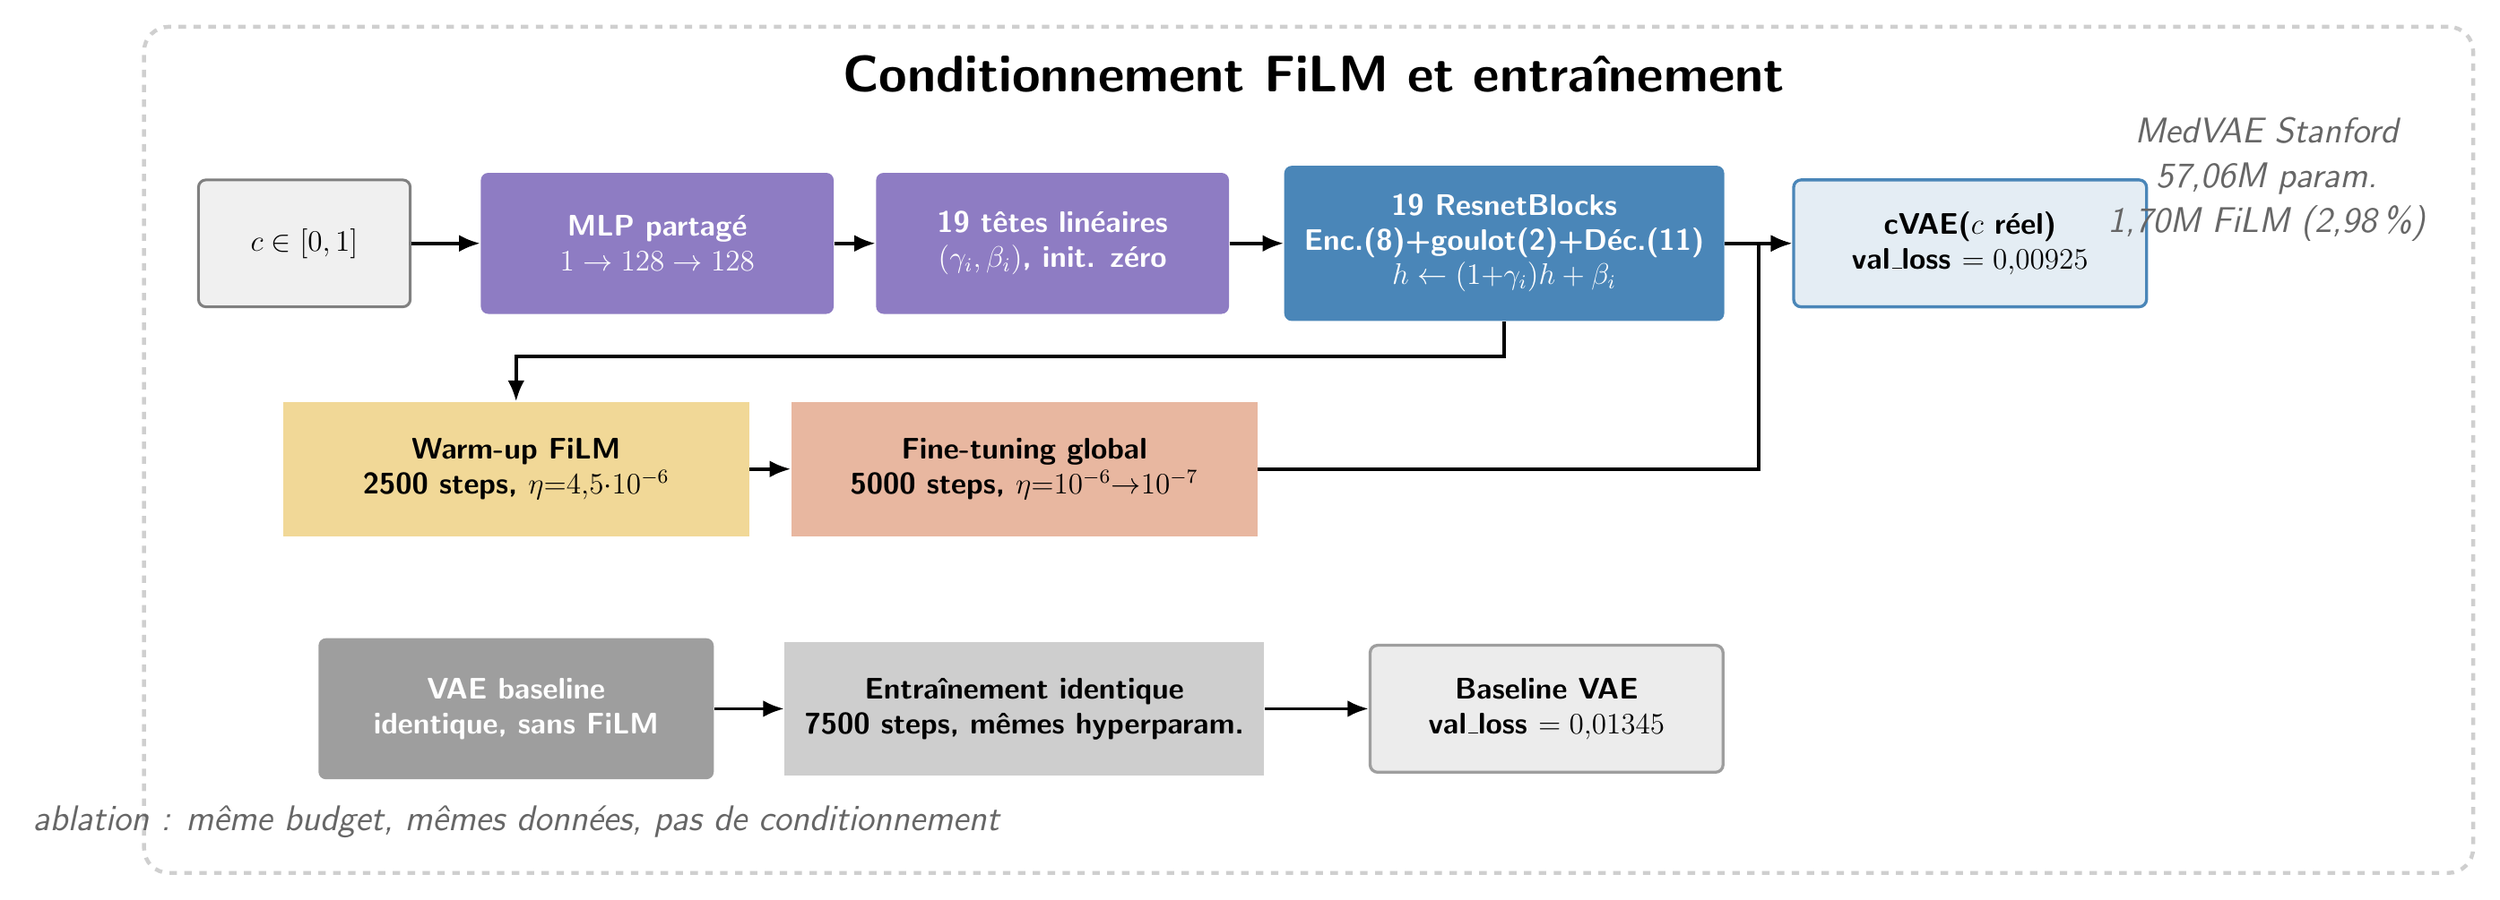
\begin{tikzpicture}[x=1cm,y=1cm]

\node[panel,minimum width=33cm,minimum height=12cm,anchor=north west] at (-.3,11.7){};

\node[title] at (16.3,11.0) {Conditionnement FiLM et entra\^inement};

\node[data] (c) at (2.0,8.6) {$c \in [0,1]$};
\node[film] (embed) at (7.0,8.6) {MLP partag\'e\\$1\to128\to128$};
\node[film] (heads) at (12.6,8.6) {19 t\^etes lin\'eaires\\$(\gamma_i,\beta_i)$, init. z\'ero};
\node[vae] (resblocks) at (19.0,8.6) {19 ResnetBlocks\\Enc.(8)+goulot(2)+D\'ec.(11)\\$h\leftarrow(1{+}\gamma_i)h+\beta_i$};
\node[ckpt,draw=medBlue,fill=medBlue!15] (cvaeckpt) at (25.6,8.6) {cVAE($c$ r\'eel)\\val\_loss $=0{,}00925$};

\draw[arrow] (c.east) -- (embed.west);
\draw[arrow] (embed.east) -- (heads.west);
\draw[arrow] (heads.east) -- (resblocks.west);
\draw[arrow] (resblocks.east) -- (cvaeckpt.west);

\node[font=\sffamily\Large\itshape,text=black!60,align=center] at (29.8,9.5)
  {MedVAE Stanford\\57,06M param.\\1,70M FiLM (2,98\,\%)};

\node[phasebox,fill=phase1] (p1) at (5.0,5.4) {Warm-up FiLM\\2500 steps, $\eta{=}4{,}5{\cdot}10^{-6}$};
\node[phasebox,fill=phase2] (p2) at (12.2,5.4) {Fine-tuning global\\5000 steps, $\eta{=}10^{-6}{\to}10^{-7}$};

\draw[arrow] (resblocks.south) -- (19.0,7.0) -- (5.0,7.0) -- (p1.north);
\draw[arrow] (p1.east) -- (p2.west);
\draw[arrow] (p2.east) -- (22.6,5.4) -- (22.6,8.6) -- (cvaeckpt.west);

\node[baserow] (basevae) at (5.0,2.0) {VAE baseline\\identique, sans FiLM};
\node[phasebox,fill=baseGray!50] (pbase) at (12.2,2.0) {Entra\^inement identique\\7500 steps, m\^emes hyperparam.};
\node[ckpt,draw=baseGray,fill=baseGray!20] (baseckpt) at (19.6,2.0) {Baseline VAE\\val\_loss $=0{,}01345$};

\draw[arrow] (basevae.east) -- (pbase.west);
\draw[arrow] (pbase.east) -- (baseckpt.west);

\node[font=\sffamily\Large\itshape,text=black!60,align=center] at (5.0,0.4)
  {ablation : m\^eme budget, m\^emes donn\'ees, pas de conditionnement};

\end{tikzpicture}
\end{document}
